% !TeX TXS-program:compile = txs:///arara
% arara: lualatex: {shell: no, synctex: yes, interaction: batchmode}
% arara: pythontex: {rerun: modified} if found('pytxcode', 'PYTHONTEX#py')
% arara: lualatex: {shell: no, synctex: yes, interaction: batchmode} if found('pytxcode', 'PYTHONTEX#py')
% arara: lualatex: {shell: no, synctex: yes, interaction: batchmode} if found('log', '(undefined references|Please rerun|Rerun to get)')

\documentclass[a4paper,11pt]{article}
\usepackage[revgoku]{cp-base}
\graphicspath{{./graphics/}}
%variables
\donnees[classe={1\up{ère} 2M2},matiere={[SPÉ.MATHS]},mois=Mai,annee=2022,typedoc=CHAP,numdoc=12]

%formatage
\author{Pierquet}
\title{\nomfichier}
\hypersetup{pdfauthor={Pierquet},pdftitle={\nomfichier},allbordercolors=white,pdfborder=0 0 0,pdfstartview=FitH}
%fancy
\lhead{\entete{\matiere}}
\chead{\entete{\lycee}}
\rhead{\entete{\classe{} - \mois{} \annee}}
\lfoot{\pied{\matiere}}
\cfoot{\logolycee{}}
\rfoot{\pied{\numeropagetot}}
\usepackage{epsdice}

\begin{document}

\pagestyle{fancy}

\part{CH12 - Variables aléatoires - Exercices}

\medskip

\begin{caide}
	{\setlength\arrayrulewidth{1.5pt} \arrayrulecolor{titrebleu!35}
		\begin{tabularx}{\linewidth}{Y|Y|Y|Y|Y|Y}
			\niveaudif{0}~~\textsf{Basique} & \niveaudif{1}~~\textsf{Modérée} & \niveaudif{2}~~\textsf{Élevée} & \niveaudif{3}~~\textsf{Très élevée} & \niveaudif{4}~~\textsf{Extrême} & \niveaudif{5}~~\textsf{Insensée} \\
	\end{tabularx}\arrayrulecolor{black}}
\end{caide}

\exonum{0}

\medskip

On tire au hasard une carte dans un jeu de 32. Dans chaque cas déterminer la loi de probabilité de la variable aléatoire $X$ qui donne le nombre de points :
\begin{enumerate}
	\item On gagne 10 points si on tire une figure, 3 points si on tire un 10, et 1 point si on tire une autre carte.
	\item On gagne 50 points si on tire l'as de trèfle, 25 points pour un autre as, 13 points si on tire le roi ou la dame de pique, 9 points pour les autres figures et on perd 37 points si on tire une autre carte.
\end{enumerate} 

\bigskip

\exonum{1}

\medskip

Calculer l'espérance $\esp{X}$, la variance $\var{X}$ et l'écart-type $\sigma(X)$ de la variable aléatoire $X$. Si besoin arrondir à $10^{-2}$.
%
\begin{multicols}{2}
	\begin{enumerate}
		\item ~
		\begin{tabularx}{5cm}{|c|Y|Y|Y|}
			\hline
			$x_i$ & $-5$ & $0$ & $7$ \\ \hline
			$P(X=x_i)$ & $0,3$ & $0,4$ & $0,3$ \\ \hline
		\end{tabularx}
		\item ~
		\begin{tabularx}{6cm}{|c|Y|Y|Y|Y|}
			\hline
			$x_i$ & $-4$ & $-3$ & $2$ & $5$ \\ \hline
			$P(X=x_i)$ & $0,2$ & $0,3$ & $0,4$ & $0,1$ \\ \hline
		\end{tabularx}
	\end{enumerate}
\end{multicols}

\bigskip

\exonum{1}

\medskip

Une urne contient les jetons, indiscernables au toucher, représentés ci-dessous.
%
\begin{center}
	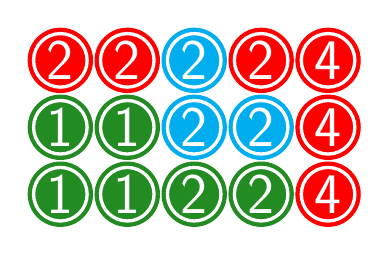
\begin{tikzpicture}[scale=0.85]
		\foreach \centre/\couleur/\numero in {%
			(0,0)/ForestGreen/1,(1,0)/ForestGreen/1,(2,0)/ForestGreen/2,(3,0)/ForestGreen/2,(4,0)/red/4,%
			(0,1)/ForestGreen/1,(1,1)/ForestGreen/1,(2,1)/cyan/2,(3,1)/cyan/2,(4,1)/red/4,%
			(0,2)/red/2,(1,2)/red/2,(2,2)/cyan/2,(3,2)/red/2,(4,2)/red/4}{%
				\filldraw[\couleur] \centre circle[radius=0.48] node[white] {\huge \sf \numero} ;
				\draw[very thick,white] \centre circle[radius=0.4] ;}
	\end{tikzpicture}
\end{center}
%
\begin{enumerate}
	\item Soit $X$ la variable aléatoire qui associe, au tirage d’un jeton dans l’urne, la valeur du nombre inscrit dessus.
	
	Déterminer la loi de probabilité de $X$.
	\item On suppose maintenant que les jetons verts comptent double, les jetons rouges comptent pour 	moitié et les jetons bleus sont sans effet. Soit $Y$ la variable aléatoire qui associe, au tirage d’un jeton dans l’urne, la valeur du nombre inscrit sur celui-ci en tenant compte des modifications.
	
	Déterminer la loi de probabilité de $Y$.
\end{enumerate}

\bigskip

\exonum{2}

\medskip

On lance simultanément deux dés cubiques équilibrés dont les faces sont numérotées de 1 à 6.

Soit $S$ la variable aléatoire qui associe à chaque lancer la somme des deux dés.
%
\begin{enumerate}
	\item Modéliser la situation à l'aide d'un tableau à double entrée.
	\begin{center}
		{\Large \renewcommand\arraystretch{1.05}\begin{tabularx}{4.5cm}{|Y|Y|Y|Y|Y|}
				\cline{2-5} 
				\multicolumn{1}{c|}{}& \epsdice{1} & \epsdice{2} & \epsdice{3} & \ldots \\ \hline
				\epsdice[black]{1} & 2 & & & \\ \hline
				\epsdice[black]{2} & & & & \\ \hline
				\ldots & & & & \\ \hline
		\end{tabularx}}
	\end{center}
	\item Déterminer la loi de probabilité de $S$.
	\item Calculer $\esp{S}$. Interpréter le résultat.
\end{enumerate}

\pagebreak

\exonum{2}

\medskip

Dans un club d’aviron, les adhérents peuvent choisir une formule d’entraînements uniquement le weekend, ou bien une formule d'entraînements le weekend et la semaine. De plus, ils peuvent adhérer au club uniquement pour accéder à toutes les installations intérieures (rameurs, salle de musculation, etc) sans profiter des 
entraînements sur l'eau. Enfin, ils ont la possibilité de s’inscrire à des séances de fitness complémentaires.

La répartition des différents adhérents est donnée dans le tableau ci-dessous :

%\begin{center}
%	\begin{tblr}{vline{1}={2-Z}{solid},vline{2-Z}={solid},hline{1}={2-Z}{solid},hline{2-Z}={solid},colspec={*{5}{Q[c,m,2.5cm]}}}
%		& {\textbf{Weekend} \\ \textbf{uniquement}} & {\textbf{Weekend} \\ \textbf{et semaine}} & \textbf{En salle} & \textbf{Total} \\
%		\textbf{Fitness} & 20 & & 70 & \\
%		\textbf{Pas fitness} & & 190 & & 350 \\
%		\textbf{Total} & 150 & & & 450 \\
%	\end{tblr}
%\end{center}
\begin{center}
	\renewcommand\arraystretch{1.25}
	\begin{NiceTabular}{W{c}{2.5cm}W{c}{2.5cm}W{c}{2.5cm}W{c}{2.5cm}W{c}{2.5cm}}[corners,hvlines]
		 & \Block[c]{}<\bfseries>{Weekend \\ uniquement} & \Block[c]{}<\bfseries>{Weekend \\ et semaine} & \Block[c]{}<\bfseries>{En salle} & \Block[c]{}<\bfseries>{Total} \\
		\textbf{Fitness} & 20 & & 70 & \\
		\textbf{Pas fitness} & & 190 & & 350 \\
		\textbf{Total} & 150 & & & 450 \\
	\end{NiceTabular}
\end{center}

\begin{enumerate}
	\item Compléter le tableau à double entrée.
	\item Le prix à l’année pour la formule weekend uniquement est de 450\,€, 505\,€ pour la formule weekend et semaine, et 400\,€ pour la formule en salle. De plus, l’inscription aux séances de fitness coûte 30\,€ par an. 
	
	On note $X$ le montant des frais d’inscription payés par un adhérent choisi au hasard dans ce club d’aviron. 
	\begin{enumerate}
		\item Déterminer les valeurs prises par $X$.
		\item Donner la loi de probabilité de $X$.
	\end{enumerate}
	\item Calculer $\esp{X}$ et interpréter le résultat.
\end{enumerate}

\bigskip

\exonum{2}

\medskip

Un restaurant propose à sa carte deux types de dessert :
%
\begin{itemize}
	\item[$\bullet~$] un assortiment de macarons, choisi par 50\,\% des clients ;
	\item une part de tarte tatin, choisie par 30\,\% des clients ;
	\item 20\,\% des clients ne prennent pas de dessert et aucun client ne prend plusieurs desserts.
\end{itemize}
%
 Le restaurateur constate :
%
\begin{itemize}
	\item que parmi les clients ayant pris un assortiment de macarons, 80\,\% prennent un café ; 
	\item que parmi les clients ayant pris une part de tarte tatin, 60\,\% prennent un café; 
	\item que parmi les clients n'ayant pas pris de dessert, 90\,\% prennent un café.
\end{itemize}
%
On interroge au hasard un client de ce restaurant. On note :
%
\begin{itemize}
	\item $M$ l'évènement : \og Le client prend un assortiment de macarons \fg{} ; 
	\item $T$ l'évènement : \og Le client prend une part de tarte tatin \fg{} ; 
	\item $P$ l'évènement : \og Le client ne prend pas de dessert \fg{} ; 
	\item $C$ l'évènement: \og Le client prend un café \fg{} et $\overline{C}$ l'évènement contraire de $C$.
\end{itemize}
%
\begin{enumerate}
	%\item En utilisant les données de l'énoncé, préciser la valeur de $p(T)$ et celle de $p_{T}(C)$.
	\item Représenter la situation par un arbre de probabilités. 
	\item  
	\begin{enumerate}
		\item Exprimer par une phrase ce que représente l'évènement $M \cap C$ puis calculer $p(M \cap C)$. 
		\item Montrer que $p(C) = \num{0,76}$.
	\end{enumerate} 
	\item Quelle est la probabilité que le client prenne un assortiment de macarons sachant qu'il prend un café ?
	\item Un assortiment de macarons est vendu 6\,€, une part de tarte tatin est vendue 7\,€, et un café est vendu 2\,€.
	
	Chaque client prend un seul plat au prix unique de 18\,€, ne prend pas plus d'un dessert ni plus d'un café.
	%
	\begin{enumerate}
		\item Quelles sont les six valeurs possibles pour la somme totale dépensée par un client? 
		\item Compléter le tableau suivant donnant la loi de probabilité de la somme totale dépensée par un client :
		%	
		\begin{center}
			\begin{tabularx}{0.7\linewidth}{|l|*{6}{>{\centering \arraybackslash}X|}}\hline
				Sommes $s_{i}$& 18 &20 &24 &\ldots&\ldots&\ldots\\ \hline
				Probas $p_i$&0,02&0,18&\ldots&&&\\ \hline 
			\end{tabularx}
		\end{center}
		\item Calculer l'espérance mathématique de cette variable aléatoire et interpréter ce résultat. 
	\end{enumerate}
\end{enumerate}

\end{document}